\documentclass[conference]{IEEEtran}
\IEEEoverridecommandlockouts
% The preceding line is only needed to identify funding in the first footnote. If that is unneeded, please comment it out.
%MMM\usepackage{cite}
\usepackage{amsmath,amssymb,amsfonts}
\usepackage{algorithmic}
\usepackage{graphicx}
\usepackage{textcomp}
\usepackage{xcolor}
\def\BibTeX{{\rm B\kern-.05em{\sc i\kern-.025em b}\kern-.08em
    T\kern-.1667em\lower.7ex\hbox{E}\kern-.125emX}}
    
    %MMM
\usepackage{biblatex} 
\usepackage[english]{babel}
\usepackage{minted}
\usepackage{fancyvrb}
\usepackage{listings}    
    %mmm
    
    
    
\bibliography{template.bib}
\usepackage{comment}
 
    
    
    
    
\begin{document}




\title{Video Streaming Mixer Library\\}
 

\author{\IEEEauthorblockN{Yuni Amaloa Quintero Villalobos}
\IEEEauthorblockA{\textit{TU Berlin} \\
\textit{Fraunhofer-FOKUS-Institut  }\\
Berlin, Germany \\
Quintero.villalobos@campus.tu-berlin.de}



\and
\IEEEauthorblockN{Mohamed Mesto}
\IEEEauthorblockA{\textit{TU Berlin} \\
\textit{Fraunhofer-FOKUS-Institut  }\\
Berlin, Germany \\
m.mesto@campus.tu-berlin.de }
\and

\IEEEauthorblockN{Poonam Kumari Roy}
\IEEEauthorblockA{\textit{TU Berlin} \\
\textit{Fraunhofer-FOKUS-Institut  }\\
Berlin, Germany \\
Poonam.k.roy@campus.tu-berlin.de}
}

\maketitle

\begin{abstract}
Adaptive Bitrate Streaming is now the standard for the biggest streaming and video player platforms online. Data is now shared over the internet dynamically, adjusting the video resolution to the user's internet capabilities to provide a better experience. In this work, we present a proof of concept to implement two strategies that join multiple video streams into a single one only if they have matching resolutions. The motivation for this research comes from the necessity to improve the user experience and to test a new way to consume media content online. To do so, we develop a library dependency with two strategies to find matching resolutions, one that only matches the resolution of the first stream in the list, and the second, the intersection of all resolutions. Our library is implemented as a Node JS package for external applications to import. Results show the Master Manifest playlist being written with all streams content concatenated in a single one. Moreover, no playback errors were presented when the video player switches between streams as long as they have the same format regarding audio tracks. 




\begin{IEEEkeywords}
video streaming, HLS, adaptive bitrate streaming, media playlist, video segments, HLS Parser, mixer library

\end{IEEEkeywords}
\end{abstract}


 

\section{\textbf{Introduction}}\label{sec:Introduction}
Adaptive streaming video standards are the norm for anything that is video and is streamed over the internet nowadays
For streaming adaptive video there are two main standards, MPEG-DASH and Apple‘s HLS – both similar in how they work
Instead of a single video file being transferred to clients, adaptive streaming works by splitting video into smaller segments, each segment being its own file. These video segment files are referenced by playlist files that specify time, duration and order of segments
By providing playlists and video segments playback becomes much more flexible and robust as it provides a number of benefits
Splitting of video and audio tracks, to e.g. provide multiple different audio tracks with different languages
Provide multiple video tracks with different resolution and bitrate to accomodate (temporary) bandwith bottlenecks during transfer
Being able to seamlessly switch between tracks to e.g. 720p, 1080p or 4K video resolution

\begin{figure}

\centering
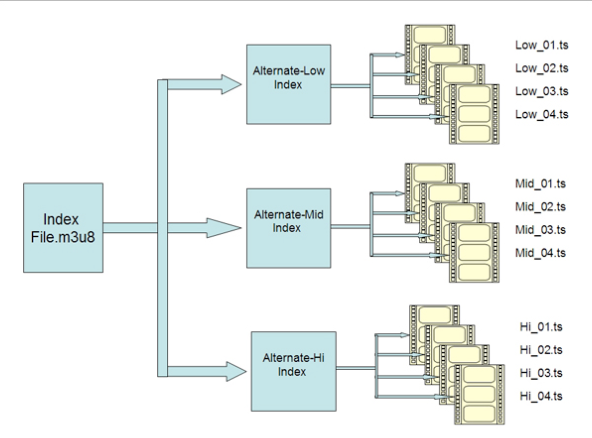
\includegraphics[scale=0.40]{figures/ProblemStatement.png}
\caption{Problem Statement \cite{rancy2016imt}}
\label{fig:IMT_2020_Use-cases}
\end{figure}


\subsection{Problem Statement
}\label{Problem Statement
}

We are in the Streaming Era

Content is transmitted without downloading

ABS dynamically changes the video source to avoid buffering

HLS splits a video file into little segments 

Not all streams share the same representations

We need an algorithm that identifies matching representation from variant video streams in order to output a single playlist












\section{\textbf{Technical Foundations}}\label{sec:techfoundation}
\subsection{Adaptive Bitrate Streaming}

Adaptive Bitrate Streaming allows broadcasters to deliver high-quality streams to users with outstanding bandwidth and processing power, while also accommodating those lacking in the speed and power departments. Rather than creating one live stream at one bitrate, a transcoder (usually located in the media server) is used to create multiple streams at different bitrates and resolutions. The server then sends the highest-resolution stream possible for each viewer’s screen and connection speed. Creating multiple renditions of a single stream helps prevent buffering or stream interruptions. Plus, as a viewer’s signal strength goes from two bars to three, the stream dynamically adjusts to deliver a superior rendition. \cite{abs}

Adaptive bitrate streaming solves each of the two main problems with progressive streaming: Quality and buffering. It allows the video provider to create a different video for each of the screen sizes (or devices) that they wish to target. If a small video can be downloaded faster than a large video, and a user has a slow internet connection, an adaptive video stream will switch to smaller video file sizes to keep the video playing. An example of this can be shown in Figure \ref{fig:abs}.

\begin{figure}[!ht]
	\centering
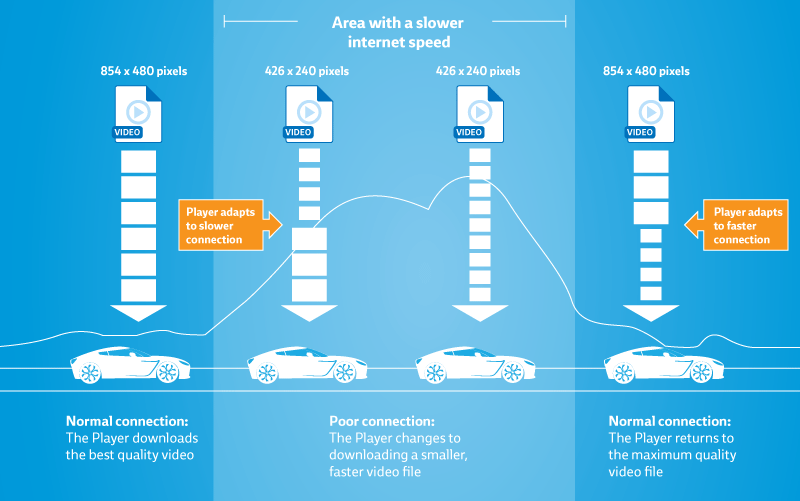
\includegraphics[scale=0.29]{figures/abs.png}\\
	\caption{Adaptive Bitrate Streaming switching video resolution \cite{abs}}
	\label{fig:abs}
\end{figure}

When a video file is encoded into an adaptive format, it is broken up into segments.
These are short snippets of video, often set to 4 seconds long (although they can be longer or shorter). At the end of each 4-second segment, the Player can switch to a different video file if necessary.

\subsection{HTTP Live Streaming}
HTTP Live Streaming (HLS) is an adaptive streaming communications protocol created by Apple. It uses the m3u8 manifest format. It provides a reliable, cost-effective means of delivering continuous and long-form video over the Internet. HLS allows a receiver to adapt the bit rate of the media to the current network conditions to maintain uninterrupted playback at the best possible quality.
  
HLS video streams are broken up into segments of data (also called chunks or packets) rather than being delivered as a continuous flow of information. To deliver the highest-quality stream possible to everyone watching, including those with small screens and poor connections, HLS streaming dynamically adapts the resolution to each individual’s circumstances. \cite{wowza}
   
In a typical HLS workflow, a video encoder solution that supports HLS receives a live video feed or distribution-ready media file. The encoder creates multiple versions (known as variants) of the audio/video at different bit rates, resolutions, and quality levels. The encoder then segments the variants into a series of small files, called media segments. At the same time, the encoder creates a media playlist file for each variant containing a list of URLs pointing to the variant’s media segments. The encoder also creates a master playlist file, containing a list of the URLs to variant media playlists, and descriptive tags to control the playback behavior of the stream. \cite{applehls} 

\subsection{Definitions}

We are going to mention some definitions \cite{refs} that will be used frequently in the upcoming sections to describe our approach. 

\subsubsection{.M3U8 Manifest File}

HLS video segments are indexed into a media playlist so that the video player understands how to organize the data. A master .m3u8 playlist file must also be created to instruct the player on how to jump between the variant-specific playlists. This is also referred to as the manifest file. \cite{wowza}

\subsubsection{Playlist}
A Playlist is either a Media Playlist or a Master Playlist.  Both are UTF-8 text files containing URIs and descriptive tags. Each Playlist file must be identified either by the path component of its URI or by HTTP Content-Type.  In the first case, the path must end with either .m3u8 or .m3u.  In the second, the HTTP Content-Type must be "application/vnd.apple.mpegurl" or "audio/mpegurl".
   
\subsubsection{Master Playlist}

A Master Playlist provides a set of Variant Streams, each of which describes a different version of the same content. A Playlist is a Master Playlist if all URI lines in the Playlist identify Media Playlists.
   
The master playlist provides an address for each media playlist in the stream. Figure \ref{fig:masterpl} shows this relationship. The master playlist also provides important details such as bandwidth, resolution, and codecs. The player uses that information to decide the most appropriate variant for the device and the currently measured, available bandwidth. \cite{applehls}

\begin{figure}[!ht]
	\centering
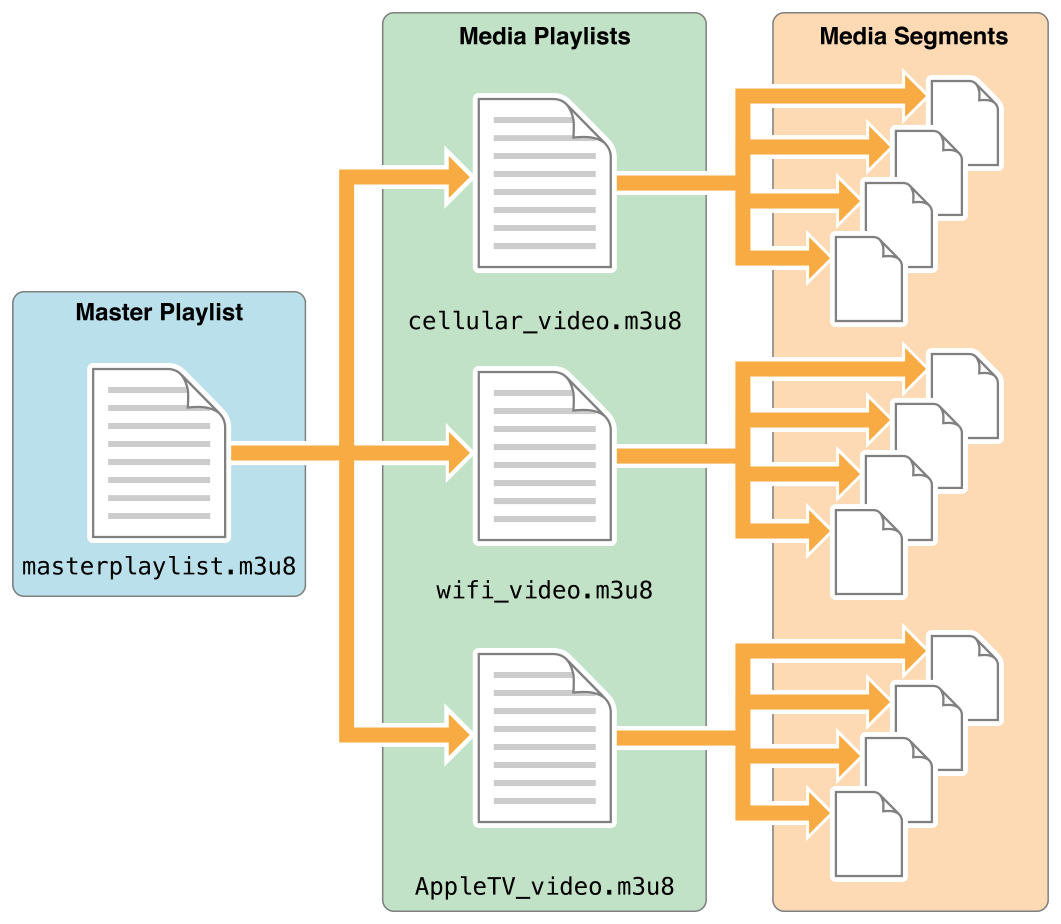
\includegraphics[scale=0.23]{figures/masterplaylist.png}\\
	\caption{Playlist relationships \cite{applehls}}
	\label{fig:masterpl}
\end{figure}
   
The following sample master playlist shows four variants. The player begins downloading the first variant it can play. If conditions warrant, the player switches to another media playlist midstream.

\begin{verbatim}
#EXTM3U
#EXT-X-VERSION:6
#EXT-X-STREAM-INF:BANDWIDTH=2855600,
RESOLUTION=960x540
live/medium.m3u8
#EXT-X-STREAM-INF:BANDWIDTH=5605600,
RESOLUTION=1280x720
live/high.m3u8
#EXT-X-STREAM-INF:BANDWIDTH=1755600,
RESOLUTION=640x360
live/low.m3u8
#EXT-X-STREAM-INF:BANDWIDTH=545600,
RESOLUTION=416x234
live/cellular.m3u8
\end{verbatim}

\subsubsection{Media Playlist}

A Media Playlist contains a list of Media Segments, which, when played sequentially, will play the multimedia presentation. The media playlists contain URLs to the media segments and other information needed for playback. 
   
Here is an example of a Media Playlist:
\begin{verbatim}
#EXTM3U
#EXT-X-TARGETDURATION:10
#EXTINF:9.009,
http://media.example.com/first.ts
#EXTINF:9.009,
http://media.example.com/second.ts
#EXTINF:3.003,
http://media.example.com/third.ts
\end{verbatim}
   
The first line is the format identifier tag \#EXTM3U. The line containing \#EXT-X-TARGETDURATION says that all Media Segments will be 10 seconds long or less.  Then, three Media Segments are declared. The first and second are 9.009 seconds long; the third is 3.003 seconds.

To play this Playlist, the client first downloads it and then downloads and plays each Media Segment declared within it. A Playlist is a Media Playlist if all URI lines in the Playlist identify Media Segments. The encoder creates the media playlists as text files saved in the M3U format (.m3u8). \cite{applehls}

\subsubsection{Variant Stream}

A Variant Stream includes a Media Playlist that specifies media encoded at a particular bit rate, in a particular format, and at a particular resolution. Clients should switch between different Variant Streams to adapt to network conditions.

\subsubsection{Renditions}

A Variant Stream can also specify a set of Renditions. Renditions are alternate versions of the content, such as audio produced in different languages.

\subsubsection{Media Segment}

A Media Playlist contains a series of Media Segments that make up the overall presentation.  A Media Segment is specified by a URI. The duration of each Media Segment is indicated in the Media Playlist by its EXTINF tag. An encoder creates media segments by dividing the event data into short MPEG-2 transport stream files (.ts). Typically, the files contain H.264 video or AAC audio with a duration of 5 to 10 seconds each. 
\section{\textbf{Related Work }}\label{sec:relatedwork}

\subsection{Dynamic ad-insertion and content orchestration workflows through manifest manipulation in HLS and MPEG-DASH}

The work presented in \cite{adinsertion} uses Manifest manipulation to dynamically insert ads into media content with the FAMIUM DAI solution. This study mentions how HLS specifies a so-called \#EXT-X-DISCONTINUITY tag, which is used in the manifest file to decorate a generic discontinuity at the source. This could be a switch of e.g. encoding parameters, input sources, or an advertisement, which has been spliced into the source. This was useful in our work to concatenate segments from different video sources, which will be explained in more detail in the Our approach section

This work has a component named The Manifest Stitcher, which performs individual manifest stitching, based on content playlists served by another entity in their architecture. The component creates MPEG-DASH and HLS manifests on the fly. The Stitcher requests the manifest files for the original content assets as well as for the pre-conditioned ad asset and creates a new manifest comprising multiple periods. This new manifest is sent to the client and allows him to play the individual stitched content.

The basic idea behind that approach is to ingest content or ads into DASH and HLS Streams by repackaging the stream. The output stream behaves like a linear stream, just like our use case for a single stream containing multiple input video streams. The re-packaged content can be handled by the player in the same way as the linear original stream. To guarantee smooth playback without re-initialization of the video player, it is necessary to condition the original stream and the content to be inserted with the same content specifications in terms of audio and video coding settings. These last conditions are also considered for our work, streams with different audio formats will not play properly.
 
\subsection{ABR streaming with separate audio and video tracks: measurements and best practices}

This paper \cite{measures} examines the state of the art in the handling of demuxed audio and video tracks in predominant Adaptive Bitrate Streaming protocols (DASH and HLS). They found several limitations in existing practices both in the protocols and the player implementations, which can cause undesirable behaviors such as stalls, selection of potentially undesirable combinations such as very low-quality video with very high-quality audio, etc. Our work had to handle streams with separate audio tracks, having to join both video and audio segments in separate manifest files without consideration on how well is the quality of experience; this matter will be covered in the Evaluation and Results section.

\subsection{Increasing ad personalization with server-side ad insertion}

This paper \cite{ssai} examines the architectures required to achieve server-side advertisement insertion so that multiple concurrent advertising manifests can be delivered in a timely fashion. Cloud and cloud-assisted software solutions were required. 

When a video plays, the player makes the necessary calls to obtain the next chunk of content to be shown from the manifest. In a well-designed player, where the segments come from the same source, there should be a seamless display and a reasonable quality of experience. What is required, then, is a method of inserting targeted advertising into individual delivery paths that provides clear metrics, protects against advertising blocking or skipping, and maintains a consistent quality of experience for the consumer. The solution lies in upstream insertion of the advertising so that a continuous stream arrives at the consumer device eliminating any possibility of discrimination between content and commercials, and avoiding freezes, black screens, and spinning wheels.

In \cite{ssai}, is shown an HLS example manifest that uses the "\#EXT-X-CUE-OUT" manifest declaration, which is the signal to the player that this is a commercial break. When using client-side advertisement insertion, the player will have some sort of logic to initiate a call to get the advertisements. The player will probably download ads to play within the time between the CUE markers. During the "\#EXT-X-CUE" breaks, it is clear that some calls are not to the content provider but advertising servers. By moving the advertising insertion to the server side and within the packaging process, the content provider address and the advertisement server provider address differences are eliminated and made to look the same from a manifest perspective. There is no need to put the \#EXT-X-CUE tags anymore as the ad insertion or replacement is already done. The client's content and the ads would be hosted at the same address. 

This eliminates the prospect of skipping the advertising, a consistent stream of content is also presented in the same resolution, codec, and encryption, which maintains the quality of experience. Finally, a single contiguous stream is sent to the client.
\section{\textbf{Our Approach}}\label{sec:main}
\subsection{ Proposed Solution}

This project was developed in Javascript programming language to be able to use hls-parse js library features, with Node JS and npm as deployment and distribution tools. 

We parsed the HLS manifests from the multiple input video streams using the hls-parse JS library. Having the respective object representations for further manipulation and handling, we implemented two algorithms that identify the matching representations based on resolution, shown in Figure \ref{fig:strategies}.

 \begin{itemize}

     \item Strategy 1: The first strategy consists of identifying which video streams have matching representations against the first element of the input array. One video stream might have more resolutions than the first input so those would be left out. As can be seen in Figure \ref{fig:strategies}, video stream B does not have the green resolution, that is present in A, so this stream is not present in the final output.

     \item  Strategy 2: The second strategy consists of finding an intersection between the variant playlists in regards to their resolution. In Figure \ref{fig:strategies} we can see that only two resolutions are common between all the input streams so an intersection has been found. Two variant playlists should be in the output manifest. Each one will include all concatenated segments from all inputs matching the respective representation.


 \end{itemize}
 
 For both strategies, the final output should be the master HLS manifest of a playlist that includes the concatenated segments from all inputs matching the respective representation. Using the hls-parser library we will create and manipulate this final HLS master manifest.

 
\begin{figure}[!ht]

\centering
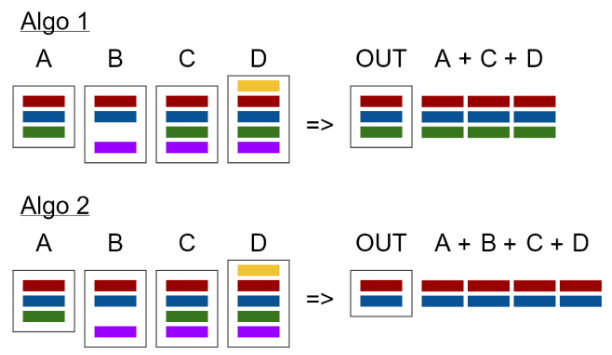
\includegraphics[scale=0.70]{figures/strategies.png}
\caption{Strategies}
\label{fig:strategies}
\end{figure}

In figure \ref{fig:proposal} we can see the diagram flow that shows how the multiple video streams manifest as input are going to be parsed through the hls-parse library to obtain each object representation, so we can handle and manipulate its data. Then, the two strategies will be applied to this set of objects to find the matching and compatible representations to output a final master playlist using, again, the hls-parse library to create/write the master manifest.

\begin{figure}[!ht]

\centering
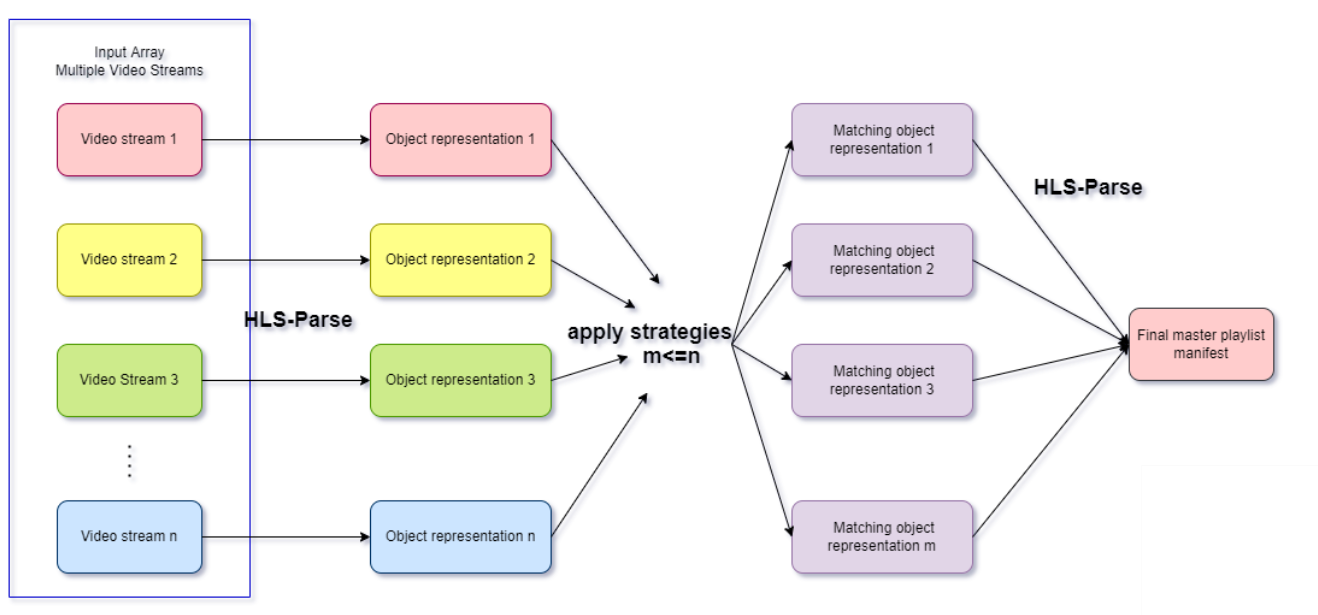
\includegraphics[scale=0.31]{figures/proposal.png}
\caption{Proposed Solution}
\label{fig:proposal}
\end{figure}

\subsection{HLS Manifest Parsing}

Each strategy receives as a parameter an array made of Strings consisting of different video stream URLs that are already .m3u8 files. To obtain the manifest text from the URLs, we fetched the data using the \Verb|fetch()| JavaScript function, which makes a GET request to the URL to obtain the text data returned. Then, we parsed the text into object representation using the hls-parser library to access the playlist as a JS object.

Hls-parser provides synchronous functions to read/write HLS playlists \cite{hlsparser}. With the method \Verb|HLS.parse(string)|, we obtained the Master playlist manifest from each URL. The object representation of a Master Playlist, its Variants, and audio tracks, look like this (simplified):

\begin{lstlisting}

MasterPlaylist {
  type: 'playlist',
  isMasterPlaylist: true,
  uri: 'https://playertest.longtailvideo.com/adaptive/elephants_dream_v4/redundant.m3u8',
  version: 3,
  source: '#EXTM3U\n' +
    '#EXT-X-MEDIA:TYPE=AUDIO,GROUP-ID="aac",LANGUAGE="en",NAME="English",DEFAULT=YES,URI="media/b160000-english.m3u8"\n' +
    '#EXT-X-STREAM-INF:BANDWIDTH=2962000,RESOLUTION=1280x720,AUDIO="aac"\n' +
    'media/b2962000-video.m3u8\n' +
    '#EXT-X-STREAM-INF:BANDWIDTH=1427000,RESOLUTION=768x432,AUDIO="aac"\n' +
    'media/b1427000-video.m3u8\n',
  variants: [
    Variant {
    uri: 'media_b/b2962000-video.m3u8',
    bandwidth: 2962000,
    resolution: { width: 1280, height: 720 },
    audio: [ 
    Rendition {
      type: 'AUDIO',
      uri: 'media/b160000-english.m3u8',
      groupId: 'aac',
      language: 'en',
      assocLanguage: undefined,
      name: 'English',
      isDefault: true,
      }
    ]
  },
    Variant {
    uri: 'media_b/b1427000-video.m3u8',
    bandwidth: 1427000,
    resolution: { width: 768, height: 432 },
    audio: [ 
    Rendition {
      type: 'AUDIO',
      uri: 'media/b160000-english.m3u8',
      groupId: 'aac',
      language: 'en',
      assocLanguage: undefined,
      name: 'English',
      isDefault: true,
      }
    ]
  }
  ],
}

\end{lstlisting}

The resolution attribute from the Variant object will be useful in finding the matching representations for each strategy. The bandwidth attribute helped us choose which representation to include when two shared the same resolution but with different bandwidths, taking the highest one. The different Uri attributes are concatenated at the end of the original address of the master playlist to later fetch the text data inside those .m3u8 files for Variant and Audio playlists.

Having the complete object representation, we saved the different Variants from each URL into a Dictionary, where the key is the index of the URL in the input URLs array and has as value an array made of the variants objects from that stream. We also saved the object representation from all the playlists in another array for later use.

\subsection{Strategy 1}

pWe need as a final output a master playlist that contains the same representations available from the first video stream of the input array. So, if we have as input array [urlA, urlB, urlC], where stream A has 360p  and 720p resolutions, stream B has 360p, 480p and 720p, and stream C has only 360p. The only stream that matched Stream A's representations was Stream B, so the final output will have Streams A and B content with 360p and 720 representations. 

We extracted the resolutions of the first element of the array from the variants dictionary mentioned before. These are our needed resolutions, then we will iterate over the other streams and for each, we will obtain its variants. We will find the needed resolution in all the representations available for every other stream. We will save the object representation of the matching streams into an array for later use.

\subsection{Strategy 2}

For strategy 2 we have as output a master playlist that contains the representations resulting from the intersection, if one exists, of all the streams variants. From the variants dictionary, we get the representations for each stream, making an array of arrays. Then, for every stream representation, we check if it exists in every other stream variant. The number of times a representation appears in the other streams to be in the intersection should equal the number of video streams minus one. If no representation is present in every stream, the intersection is empty.

So, if we have as input array [urlA, urlB, urlC], where stream A has 720p and 360p resolutions, stream B has 480p and 360p and stream C has only 360p, an intersection exists and the Master Playlist will consist of only the 360p representation of Stream A, B and C contents.

\subsection{Output final master manifest}

After implementing both strategies, we have as a result an array with the compatible streams and an array with the resolutions that matched.
Having the streams resulting from the filtering of the strategies, we have to obtain the variants for each matching resolution.

With the help of a dictionary with key the resolution as string representation 00x00, we gather all the variants that matched it according to the strategy. A stream can have multiple variants with the same resolution but with different bandwidths. To remove these duplicates, we chose the variant with the maximum bandwidth value.

For each matching resolution, we fetch the media playlist of all the variants to obtain their segments which will be joined in an array to create a new Media Playlist object that will represent the correspondent Variant representation in the final master manifest. We convert this new Media Playlist object into string representation in a .m3u8 file identified with the corresponding resolution using \Verb|HLS.stringify()| method

\begin{lstlisting}
let newPlaylist = new MediaPlaylist({
    segments: segments,
    endlist: true,
    targetDuration: maxDuration,
    version: maxVersion
})
const content = HLS.stringify(newPlaylist)
fs.writeFile(resolution + '.m3u8', content)
\end{lstlisting}

Then, we create a new Variant object that has as Uri attribute the filename of the media playlist m3u8 file mentioned before, its resolution, and bandwidth attributes, which is the maximum of all the variants joined. This new Variant object will be saved in the variants dictionary mentioned before in the corresponding resolution key as 00x00 format.

\begin{lstlisting}
let newVariant = new Variant({
    uri: resolution + '.m3u8',
    resolution: res,
    bandwidth: maxBand
})
repDict[resolution] = newVariant
\end{lstlisting}

If the matching streams have audio tracks, these will also be fetched from the correspondent .m3u8 files of the audio media playlist. Each audio segment will be saved in an array, accumulating audio from all the streams belonging to a Variant. The attribute audio for the new Variant object will have as value this audio segments array. At the same time, a new audio.m3u8 file is written which will include the audio for the final resulting stream. 
\begin{lstlisting}
let newAudioPlaylist = new MediaPlaylist({
    segments: audioSegments,
    endlist: true,
    targetDuration: maxAudioDuration,
    version: maxAudioVersion
})
const content = HLS.stringify(newAudioPlaylist)
fs.writeFile('audio.m3u8', content)
let audio = new Rendition({
    type: 'AUDIO',
    uri: 'audio.m3u8',
    groupId: 'audio',
    name: 'audio'
})
newVariant.audio = [audio]
\end{lstlisting}
Finally, we create a new MasterPlaylist object joining all the variants in the dictionary in an array to assign the variants attribute to the master playlist. We convert this playlist into string representation too and write it on a master.m3u8 file.

\begin{lstlisting}
let masterPlaylist = new MasterPlaylist({
    variants: variants
})
HLS.stringify(masterPlaylist)
fs.writeFile('master.m3u8', content)
\end{lstlisting}

\subsection{Dependency Library}

The final requirement for this project was to deploy it as a dependency for other Node JS applications to use.

We created a npm package \cite{npm}, which has in the file utils.js two methods: \Verb|algorithmA()| and \Verb|algorithmB()|, where both receive as parameters an array of string URLs, along with other utility functions like \Verb|joinSegments()|, \Verb|makeRepresentationsDict()|, \Verb|createMasterPlaylist()|. These two methods, \Verb|algorithmA()| and \Verb|algorithmB()|, are exported in the index.js of the package from which an external Node JS app can import them as a dependency.
\section{\textbf{Results and Discussion}}\label{sec:Evaluation} 

To test the Master Manifests, Safari Web Browser was used as it has native HLS support in its video player. The VLC video player was an option but it produced playback errors when switching streams, the player restarted the counter instead of having continuity. Native HLS Playback Google Chrome extension was also tested, but it produced playback errors between streams. Safari had the best performance for testing. The idea is to have the streams mixed into a single stream playing sequentially.

Because we are writing the master manifest in a local file on our computer, we need a localhost server running so the videos can be played in Safari. We used the following python command in the Unix environment:  \Verb|python3 -m http.server|
To play the stream in the Safari search bar, one types \textcolor{blue}{http://localhost:8000/master.m3u8}

We also have a Node JS testing application which will serve us as our external application and imports the video mixer library as a dependency. This application has a main.js file that calls the \Verb|algorithmA()| and \Verb|algorithmB()| methods.

\subsection{Strategy 1}

We tested the first strategy, which consists of having as an output a final manifest that will have the representations present only for the first element of the input array. In this case, we made an HLS file which is hosted in our computer for testing purposes. The Node JS application calls the first strategy method with three input streams:

\begin{lstlisting}
algorithmA(["http://localhost:8000/puskasStream/master.m3u8",
    "https://playertest.longtailvideo.com/adaptive/oceans_aes/oceans_aes.m3u8",
    "https://test-streams.mux.dev/pts_shift/master.m3u8"])
\end{lstlisting}

The three streams have respectively these resolutions: 

\begin{itemize}
\item 1280x720
\item 304x128, 384x160, 544x224, 736x304, 960x400, 1264x528
\item 480x270, 768x432, 864x486, 1280x720
\end{itemize}

Once the localhost server was running, we tested the first strategy. The first URL's resolution, which is the needed resolution, is 1280x720 and it is not present in the second stream but it is in the third one. Our final manifest as an output from the algorithm will have only one variant which is 1280x720 and makes a reference to the media playlist file that was created for this representation. The playlist file has all the segments from the two streams concatenated in a single list.

Here is the resulting Master Manifest which has the only resolution present in the first input stream, 1280x720. This variant has a media playlist and it does not include an audio track because the video segments have them integrated.

\begin{lstlisting}
#EXTM3U
#EXT-X-STREAM-INF:BANDWIDTH=2320000,
RESOLUTION=1280x720
1280x720.m3u8
\end{lstlisting}

Here is the media playlist manifest (simplified) for the 1280x720 resolution. This playlist has all the video segments from the two streams concatenated in a single list. In between the two streams, the \#EXT-X-DISCONTINUITY tag has to be inserted.

\begin{lstlisting}
#EXTM3U
#EXT-X-VERSION:3
#EXT-X-TARGETDURATION:16
#EXT-X-DISCONTINUITY
#EXTINF:11.533333,
http://localhost:8000/puskasStream/All Puskas Award Winners (2009-2021)0.ts
#EXTINF:8.5,
http://localhost:8000/puskasStream/All Puskas Award Winners (2009-2021)1.ts
...
#EXT-X-DISCONTINUITY
#EXTINF:4.736,
https://test-streams.mux.dev/pts_shift/media-uoj0it22v_0.ts
#EXTINF:4.8,
https://test-streams.mux.dev/pts_shift/media-uoj0it22v_1.ts
...
\end{lstlisting}

\subsection{Strategy 2}

We tested the second strategy, which consists of the intersection of resolutions from the input URLs. The Node JS application calls the second strategy method with two input streams: 

\begin{lstlisting}
algorithmB(["http://amssamples.streaming.mediaservices.windows.net/634cd01c-6822-4630-8444-8dd6279f94c6/CaminandesLlamaDrama4K.ism/manifest(format=m3u8-aapl)", 
    "http://amssamples.streaming.mediaservices.windows.net/91492735-c523-432b-ba01-faba6c2206a2/AzureMediaServicesPromo.ism/manifest(format=m3u8-aapl)"])
\end{lstlisting}

The two streams have respectively these resolutions: 

\begin{itemize}
\item 640x360, 960x540, 1280x720, 1920x1080, 2560x1440, 3840x2160, 4096x2304
\item 320x180, 640x360, 960x540, 1280x720, 1920x1080
\end{itemize}

The intersection of all resolutions is: 640x360, 960x540, 1280x720 and 1920x1080

For simplicity, we are going to call Stream1 and Stream2 to replace the URLs in the video segments addresses, also, we are not listing the complete playlist.

We can see that for these three streams we have four representations resulting from the intersection. The representations 640p, 960p, 1280p, and 1920p are present in these three streams. We have as output files four representations along with the master manifest. We can see that our master manifest has now four variants, each of them referring to the media playlist file which has the name of the resolution. We have all the segments or clips concatenated for the three streams.

Here is the resulting Master Manifest from the intersection of the resolutions from the input streams. Four variants are present, each with its m3u8 playlist manifest. The two matching streams each had audio tracks themselves, so each variant refers to the audio track.

\begin{lstlisting}
#EXTM3U
#EXT-X-MEDIA:TYPE=AUDIO,GROUP-ID="audio",
NAME="audio",URI="audio.m3u8"
#EXT-X-STREAM-INF:BANDWIDTH=1355199,
RESOLUTION=640x360,AUDIO="audio"
640x360.m3u8
#EXT-X-STREAM-INF:BANDWIDTH=2532741,
RESOLUTION=960x540,AUDIO="audio"
960x540.m3u8
#EXT-X-STREAM-INF:BANDWIDTH=2532741,
RESOLUTION=1280x720,AUDIO="audio"
1280x720.m3u8
#EXT-X-STREAM-INF:BANDWIDTH=2532741,
RESOLUTION=1920x1080,AUDIO="audio"
1920x1080.m3u8
\end{lstlisting}

Here is the audio playlist manifest (simplified). This playlist has all the audio segments from the two streams concatenated in a single list. In between the two streams, the \#EXT-X-DISCONTINUITY tag has to be inserted.

\begin{lstlisting}
#EXTM3U
#EXT-X-VERSION:4
#EXT-X-TARGETDURATION:11
#EXT-X-DISCONTINUITY
#EXTINF:10.026667
Stream1/QualityLevels(384000)/Fragments(aac_UND_6_384=100266666,format=m3u8-aapl)
#EXTINF:10.026667
Stream1/QualityLevels(384000)/Fragments(aac_UND_6_384=200533333,format=m3u8-aapl)
...
#EXT-X-DISCONTINUITY
#EXTINF:10.10068
Stream2/QualityLevels(53620)/Fragments(AAC_und_ch2_56kbps=101006802,format=m3u8-aapl)
#EXTINF:10.10068
Stream2/QualityLevels(53620)/Fragments(aac_UND_6_384=300800000,format=m3u8-aapl)
...
\end{lstlisting}

Here is the media playlist manifest (simplified) for the 640x360 resolution. This playlist has all the video segments from the two streams concatenated in a single list. In between the two streams, the \#EXT-X-DISCONTINUITY tag has to be inserted.

\begin{lstlisting}
#EXTM3U
#EXT-X-VERSION:4
#EXT-X-TARGETDURATION:11
#EXT-X-DISCONTINUITY
#EXTINF:10
Stream1/QualityLevels(926058)/Fragments(video=100000000,format=m3u8-aapl)
#EXTINF:10
Stream1/QualityLevels(926058)/Fragments(video=200000000,format=m3u8-aapl)
...
#EXT-X-DISCONTINUITY
#EXTINF:10.01
Stream2/QualityLevels(642832)/Fragments(video=100100000,format=m3u8-aapl)
#EXTINF:10.01
Stream2/QualityLevels(642832)/Fragments(video=200200000,format=m3u8-aapl)
..
\end{lstlisting}

\subsection{Discussion}

We can see that every time a playlist switches to a different content source (different stream), we add the \#EXT-X-DISCONTINUITY tag. The EXT-X-DISCONTINUITY tag indicates a discontinuity between the Media Segment that follows it and the one that preceded it. The EXT-X-DISCONTINUITY tag must be present if there is a change in file format or encoding parameters \cite{refs}. The client must be prepared to reset its parser and decoder before playing a Media Segment that has an EXT-X-DISCONTINUITY tag applied to it; otherwise, playback errors can occur. During the testing phase, when the tag was not present, the playback was failing when the player tried to switch to the next stream.
   
One use-case this project did not cover was mixing a stream that has audio tracks with one that doesn't. This would require, for future work, playing the audio playlist only in its correspondent video timestamp. It is assumed that timestamp manipulation is supported in HLS. Without timestamp manipulation, the stream that has audio integrated into each video segment plays with audio normally, when the player switches to the next stream, it has no audio because it depends on the audio tracks that were left out.

Additionally, if audio tracks are present in all matching streams, only one audio track is being included, for example, English audio. If other languages were available, the video mixer library would only choose the default audio.
\section{\textbf{Conclusions}}\label{sec:conclusions}

As a result of this project, users can enjoy, for example, a complete TV series in a single sit without interrupting the experience by refreshing the page for the next episode. Multiple streams can be played as a single one as long as they have matching resolutions and audio format.

This last feature is a future work that needs to be implemented and is considered a limitation in this present proof of concept as mentioned in the Discussion section, as well as multiple audio support where the user can choose, for example, which language audio to play.

Hls-parser was easy to work with and very intuitive. Some challenges were present when playlist URLs are in relative path format, so they had to be parsed and joined with the original stream address. In the initial stages of testing, video playback errors were present until further research discovered that the Discontinuity tag, mentioned in the Results section, was needed to have a smooth transition between streams.

The video mixer library leads to the beginning of a new era of streaming technologies, having as a goal to improve the user experience and, tentatively, to attach them to the web page for them to be exposed to more ads which leads to market profits.








%mmm\section*{References}

 





    %\bibliographystyle{IEEEtran} % enable for bibtex
    % enable for bibtex
    \printbibliography% enable for biber style
    % to show unreferenced publications ------------------------------------- */
    %\bibliographystyle{unsrt}
    %\cite{dummy}
    %\nocite{*}
    %------------------------------------------------------------------------ */

    % /* -------------------------------------------------------------------- */
    %\backmatter



\end{document}
